\documentclass{beamer}
\usepackage[T1]{fontenc}
\usepackage[utf8]{inputenc}
\usepackage[spanish]{babel}
\usepackage{lmodern}
\usepackage{algorithmic, algorithm, listings, tikz}
\usepackage{circuitikz}



\usetikzlibrary{arrows.meta}
\usetikzlibrary{shapes.geometric, arrows, positioning}

\definecolor{nubankpurple}{RGB}{130, 10, 209}
\definecolor{lambdaorange}{RGB}{255, 140, 0}
\definecolor{codegreen}{rgb}{0,0.6,0}
\definecolor{codegray}{rgb}{0.5,0.5,0.5}
\definecolor{codepurple}{rgb}{0.58,0,0.82}
\definecolor{backcolour}{rgb}{ 150 , 150 , 150 }
\definecolor{handwriting}{rgb}{0.6, 0.2, 0.2}

\lstset{
    language=Java,
    backgroundcolor=\color{backcolour},   
    commentstyle=\color{codegreen},
    keywordstyle=\color{magenta},
    numberstyle=\tiny\color{codegray},
    stringstyle=\color{codepurple},
    basicstyle=\ttfamily\scriptsize,
    breakatwhitespace=false,         
    breaklines=true,                 
    captionpos=b,                    
    keepspaces=true,                 
    showspaces=false,                
    showstringspaces=false,
    showtabs=false,                  
    tabsize=2
}

\lstdefinelanguage{Clojure}{
    morekeywords={defn, def, fn, if, let, do, str, println, assoc, conj, first, rest},
    sensitive=true,
    morecomment=[l]{;},
    morestring=[b]",
}

% Use Unipd as theme
\usetheme[pageofpages=of,logo=logo_semillero_fp.png]{Unipd}

\title{Sesión 2:  Funciones Puras e Inmutabilidad}
\subtitle{Semillero en Ciencias de la Computación}
\author[Rodríguez, López]{Tomás Rodríguez \and Santiago López}

\date{Mayo 8, 2026}

% The next block of commands puts the table of contents at the beginning of each section and highlights the current section
\AtBeginSection[]
{
  \begin{frame}
    \frametitle{Tabla de Contenidos}
    \tableofcontents[currentsection,hideothersubsections,sectionstyle=show/hide]
  \end{frame}
}

\begin{document}

\frame{\titlepage}

\begin{frame}{Tabla de contenidos}
    \tableofcontents
\end{frame}

\section{Conceptos Teóricos}

\subsection{Funciones Puras}
\begin{frame}{Funciones Puras}
    Recordemos la siguiente definición:
    \begin{block}{Definición:}
        Una función se dice \textit{pura} si cumple con:
    \begin{enumerate}
        \item \textbf{Retorna un solo valor}.
        \item \textbf{El resultado depende únicamente de sus argumentos}.
        \item \textbf{No muta ningún valor existente} (cero efectos secundarios).
    \end{enumerate}
    
    \end{block}
    
    
    \vspace{0.5cm}
    
        Si las funciones puras componen el motor de los programas funcionales, los valores inmutables son su \textbf{combustible}, \textbf{aceite} y \textbf{gases}.
    
\end{frame}

\subsection{Inmutabilidad}
\begin{frame}{Inmutabilidad}
    
    \begin{block}{Definición:}
     Una vez que un dato es creado, \textbf{no puede ser cambiado}.    
    \end{block}
        
    En lugar de modificar un valor, las funciones puras \textbf{hacen copias de los datos y las pasan como resultado}.


    \vspace{0.3cm}
    \begin{center}
        \begin{tikzpicture}[node distance=1.5cm, auto, thick]
            \node[draw, rounded corners, fill=blue!10, text width=2cm, align=center] (val1) {Valor Inmutable};
            \node[draw, circle, fill=lambdaorange!30, right=of val1] (fun) {$f(x)$};
            \node[draw, rounded corners, fill=green!10, text width=2cm, align=center, right=of fun] (val2) {Nuevo Valor Inmutable};

            \draw[->] (val1) -- (fun);
            \draw[->] (fun) -- (val2);
        \end{tikzpicture}
    \end{center}
\end{frame}

\begin{frame}{Programación funcional}

    Los conceptos de función pura e inmutabilidad son tan expresivos que la programación funcional en sí misma se puede definir en únicamente estos términos:

    \vspace{0.5cm}

    \begin{block}{Definición}
        \textbf{Programación funcional} es programar usando \textit{funciones puras} que manipulan valores \textit{inmutables}.
    \end{block}
    
\end{frame}

\begin{frame}{Estudio de caso}

    Suponga que está planeando un eurotrip con sus amigos el cual luce así:

    \begin{figure}
        \centering
        \resizebox{\textwidth}{!}{%
        \begin{circuitikz}
        \tikzstyle{every node}=[font=\fontsize{18.2pt}{23.7pt}\selectfont]
        
        \node [inner xsep=0.080cm, inner ysep=0.085cm, rounded corners=0.020cm] at (1.875,11.75) {Paris};
        \node [inner xsep=0.080cm, inner ysep=0.085cm, rounded corners=0.020cm] at (4.75,11.75) {Berlin};
        \node [inner xsep=0.080cm, inner ysep=0.085cm, rounded corners=0.020cm] at (8,11.75) {Kraków};
        
        \draw (1.875,11) to[short] (8.25,11);
        
        \begin{scope}[transparency group, opacity=1]
        \node at (1.875,11) [circ, color={rgb,255:red,0; green,0; blue,0}] {};
        \end{scope}
        \begin{scope}[transparency group, opacity=1]
        \node at (4.75,11) [circ, color={rgb,255:red,0; green,0; blue,0}] {};
        \end{scope}
        \begin{scope}[transparency group, opacity=1]
        \node at (8.25,11) [circ, color={rgb,255:red,0; green,0; blue,0}] {};
        \end{scope}
        \end{circuitikz}
        }%
        \caption{Ruta de ciudades}
        \label{fig:ruta_ciudades}
    \end{figure}

\end{frame}

\begin{frame}[fragile]{Estudio de caso}
    Manjeamos nuestro itinerario así:
    
    \begin{lstlisting}[language=Java]
        List<String> planA = new ArrayList<>();
        planA.add("Paris");
        planA.add("Berlin");
        planA.add("Kraków");
        System.out.println("Plan A: " + planA);
    \end{lstlisting}

    Lo cual produce:
    \begin{verbatim}
    Plan A: [Paris, Berlin, Kraków]
    \end{verbatim}

\end{frame}

\begin{frame}{Un amigo inconveniente}
    
    Sin embargo, uno de nuestros amigos es un gran fan de Mozart el cual insiste en visitar Vienna antes de ir a Kraków.
    
    \vspace{0.5cm}
    
    \begin{block}{Ejercicio}
         Proponga una función para implementar este cambio en el itinerario.
    \end{block}
    
\end{frame}


\begin{frame}[fragile]{El Peligro de la Mutabilidad}
    Considere esta solución a la modificación del itinerario
    
    \begin{lstlisting}[language=Java]
    // Tipo de retorno inofensivo...
    static List<String> replan(List<String> plan, String newCity, String beforeCity) {
        int newCityIndex = plan.indexOf(beforeCity);
        plan.add(newCityIndex, newCity);
        return plan;
    }
    \end{lstlisting}

    \begin{enumerate}
        \item ¿Qué está haciendo la función?
        \item ¿Qué tipo de dato está devolviendo?
        \item ¿Es una función pura?
    \end{enumerate}
    
\end{frame}

\begin{frame}[fragile]{El Peligro de la Mutabilidad}
    Considere esta solución a la modificación del itinerario
    
    \begin{lstlisting}[language=Java]
    // Tipo de retorno inofensivo...
    static List<String> replan(List<String> plan, String newCity, String beforeCity) {
        int newCityIndex = plan.indexOf(beforeCity);
        plan.add(newCityIndex, newCity);
        return plan;
    }
    \end{lstlisting}
    
    \begin{alertblock}{¿Qué pasa aquí?}
        Aunque la función promete devolver un plan nuevo, en realidad muta la lista original en memoria que se le pasó como argumento. Mentir en la firma rompe nuestra intuición y es una de las mayores causas de bugs.
    \end{alertblock}
    
\end{frame}


\begin{frame}[fragile]{El Peligro de la Mutabilidad}
    Muchas preguntas surgen al observar estos comportamientos en funciones:

    \begin{figure}
        \centering
        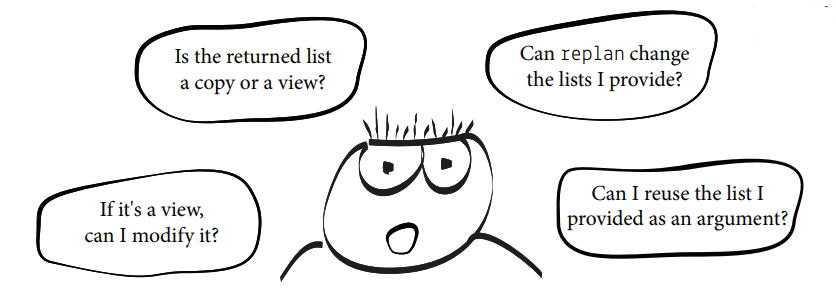
\includegraphics[width=1\linewidth]{figs/image.png}
        \caption{Los valores mutables son confusos.}
        \label{fig:placeholder}
    \end{figure}
    
\end{frame}

\begin{frame}[fragile]{Una solución}

    Considere esta modificación de replan

    \begin{lstlisting}[language=Java]
    static List<String> replan(List<String> plan, String newCity, String beforeCity) {
        int newCityIndex = plan.indexOf(beforeCity); 
        // Creamos una copia de la lista original
        List<String> replanned = new ArrayList<>(plan); 
        replanned.add(newCityIndex, newCity);
        return replanned;
    }
    \end{lstlisting}

    \begin{enumerate}
        \item ¿Es esta función pura?
        \item ¿Es esto un ejemplo de programación funcional?
    \end{enumerate}
    
\end{frame}

\begin{frame}[fragile]{Una solución}

    Considere esta modificación de replan

    \begin{lstlisting}[language=Java]
    static List<String> replan(List<String> plan, String newCity, String beforeCity) {
        int newCityIndex = plan.indexOf(beforeCity); 
        // Creamos una copia de la lista original
        List<String> replanned = new ArrayList<>(plan); 
        replanned.add(newCityIndex, newCity);
        return replanned;
    }
    \end{lstlisting}

    Es pura!!

    \begin{block}{Definición:}
        Una función se dice \textit{pura} si cumple con:
    \begin{enumerate}
        \item \textbf{Retorna un solo valor}.
        \item \textbf{El resultado depende únicamente de sus argumentos}.
        \item \textbf{No muta ningún valor existente} (cero efectos secundarios).
    \end{enumerate}
    
    \end{block}
    
\end{frame}

\begin{frame}[fragile]{Una solución}

    Considere esta modificación de replan

    \begin{lstlisting}[language=Java]
    static List<String> replan(List<String> plan, String newCity, String beforeCity) {
        int newCityIndex = plan.indexOf(beforeCity); 
        // Creamos una copia de la lista original
        List<String> replanned = new ArrayList<>(plan); 
        replanned.add(newCityIndex, newCity);
        return replanned;
    }
    \end{lstlisting}

    \textbf{No es programación funcional.} ¿Por qué?
    \begin{block}{Definición}
        \textbf{Programación funcional} es programar usando \textit{funciones puras} que manipulan valores \textit{inmutables}.
    \end{block}
    
\end{frame}


\begin{frame}[fragile]{Una solución}

    Considere esta modificación de replan

    \begin{lstlisting}[language=Java]
    static List<String> replan(List<String> plan, String newCity, String beforeCity) {
        int newCityIndex = plan.indexOf(beforeCity); 
        // Creamos una copia de la lista original
        List<String> replanned = new ArrayList<>(plan); 
        replanned.add(newCityIndex, newCity);
        return replanned;
    }
    \end{lstlisting}

    
    \begin{block}{Transparencia Referencial}
        \small
        Al no mutar argumentos externos, podemos llamar la función múltiples veces con los mismos argumentos y siempre obtener el mismo resultado.
    \end{block}
    
\end{frame}

\begin{emptyframe}
    ¿Qué tan complicada puede ponerse la mutabiliad? 
    \vspace{1cm}
    
    
    Stay tuned!!
\end{emptyframe}


\subsection{Estado mutable compartido}

\begin{frame}{Estado mutable compartido}

    Para ver que tan complicado puede volverse pensar en valores que van cambiando introducimos las siguientes definiciones:

    \begin{block}{Definición}
        Un \textbf{estado} es una instancia de un valor que está almacenado en un lugar y puede ser consultado por código.
    \end{block}
    
    \begin{block}{Definición}
        Cuando un estado puede ser modificado, tenemos un estado mutable.
    \end{block}
    
    \begin{block}{Definición}
        Cuando un estado mutable puede ser accedido por diferentes parte del código tenemos un estado mutable compartido.
    \end{block}


\end{frame}

\begin{frame}{Estado mutable compartido}

    Veamos el problema de un estado mutable compartido en acción.
    
\end{frame}

\begin{frame}[fragile]{El Escenario: Tiempos de Vuelta}
    Queremos analizar los tiempos de las vueltas de un coche de carreras. Tenemos una lista con los tiempos y necesitamos calcular:
    \begin{enumerate}
        \item El \textbf{tiempo total} de la carrera (ignorando la primera vuelta, que es de calentamiento).
        \item El \textbf{tiempo promedio} de todas las vueltas.
    \end{enumerate}

    \vspace{0.3cm}
    \begin{exampleblock}{Estado Inicial en Java}
        \begin{lstlisting}
        ArrayList<Double> lapTimes = new ArrayList<>();
        lapTimes.add(31.0); // Vuelta de calentamiento
        lapTimes.add(20.9);
        lapTimes.add(21.1);
        lapTimes.add(21.3);
        \end{lstlisting}
    \end{exampleblock}
\end{frame}

\begin{frame}[fragile]{Implementación de la solución}
    Creamos nuestra función para calcular el tiempo total. Para ignorar la vuelta de calentamiento, simplemente la eliminamos de la lista.

    \begin{lstlisting}
    static double totalTime(List<Double> lapTimes) {
        lapTimes.remove(0); // Removemos la vuelta de calentamiento
        
        double sum = 0;
        for (double x : lapTimes) {
            sum += x;
        }
        return sum;
    }
    \end{lstlisting}

       Creamos nuestra función para calcular el tiempo promedio.

    \begin{lstlisting}
    static double avgTime(List<Double> lapTimes) {
        double time = totalTime(lapTimes);
        int laps = lapTimes.size();
        return time / laps;
    }
    \end{lstlisting}

    
\end{frame}

\begin{frame}[fragile]{El Impacto de la Mutabilidad: Resultados Incoherentes}
    Definimos la lista y corremos las funciones en orden:
    \begin{columns}
        \begin{column}{0.6\textwidth}
            \begin{lstlisting}[language=Java, title={Ejecución secuencial}]
System.out.println(totalTime(lapTimes));
// -> Resultado: 63,3

System.out.println(avgTime(lapTimes));
// -> Resultado: 21.2 (<-- ¿Es esto correcto?)
            \end{lstlisting}
        \end{column}
        \begin{tikzpicture}[
        node distance=0.8cm and 0.5cm, % Reducimos un poco la separación horizontal
        box/.style={draw, rounded corners, fill=gray!20, text width=2.5cm, align=left, font=\scriptsize}, 
        arrow/.style={->, thick, >=stealth}, 
        mutation/.style={->, thick, >=stealth, red, dashed, font=\tiny}
    ]
        \begin{column}{0.35\textwidth}
            \node[anchor=west] (state1) at (0,0)
        \node[box, below=0.3cm of state1.south west, anchor=north west, fill=blue!10] (ref1) {\texttt{lapTimes}};
        \node[below =of ref1] (list1) {\fbox{31.0} \fbox{20.9} \fbox{21.1} \fbox{21.3}};
        \draw[arrow] (ref1) -- (list1);
        \end{column}
         \end{tikzpicture}
    \end{columns}

    \begin{alertblock}{Problema Oculto}
        \texttt{totalTime} tiene un \textbf{efecto secundario}: está mutando la lista original que se le pasó como argumento.
    \end{alertblock}
\end{frame}

\begin{frame}{¿Por qué falla? Rastreando el Estado Mutable Compartido}

    % \resizebox asegura que todo el diagrama se ajuste al ancho de la diapositiva (\linewidth)
    \resizebox{\linewidth}{!}{
    \begin{tikzpicture}[
        node distance=0.8cm and 0.5cm, % Reducimos un poco la separación horizontal
        box/.style={draw, rounded corners, fill=gray!20, text width=2.5cm, align=left, font=\scriptsize}, 
        arrow/.style={->, thick, >=stealth}, 
        mutation/.style={->, thick, >=stealth, red, dashed, font=\tiny}
    ]

        % --- PASO 1 ---
        % Forzamos la alineación a la izquierda fijando x=0 y usando anchor=west
        \node[anchor=west] (state1) at (0,0) {\textbf{Estado 1: Inicio}};
        \node[box, below=0.3cm of state1.south west, anchor=north west, fill=blue!10] (ref1) {\texttt{lapTimes}};
        \node[right=of ref1] (list1) {\fbox{31.0} \fbox{20.9} \fbox{21.1} \fbox{21.3}};
        \draw[arrow] (ref1) -- (list1);
        

        % --- PASO 2 ---
        \node[anchor=west] (state2) at (0,-2.5) {\textbf{Estado 2: Ejecución de \texttt{totalTime}}};
        \node[box, below=0.3cm of state2.south west, anchor=north west, fill=nubankpurple!20] (fn1) {\texttt{totalTime(lapTimes)}};
        \node[right=of fn1] (list2) { \fbox{20.9} \fbox{21.1} \fbox{21.3}};
        \draw[arrow] (fn1) -- (list2);
        % Visual mutation indicator
        \draw[mutation] (fn1) -- node[above, sloped] {.remove(0)} (list2.west);
        \node[right=of list2, text width=3.2cm] (desc1) {\small \texttt{totalTime} lee esta lista.\\ Resultado: 63.3};
        % \node[above=of desc1, text width=3.2cm, color=red] (desc2) {\small La función \textbf{modifica} el objeto en memoria!};

        % --- PASO 3 ---
        \node[anchor=west] (state3) at (0,-5.0) {\textbf{Estado 3: Ejecución de \texttt{avgTime}}};
        \node[box, below=0.3cm of state3.south west, anchor=north west, fill=red!10] (ref2) {\texttt{avgTime(lapTimes)}};
        \node[right=of ref2] (list3) { \fbox{21.1} \fbox{21.3}};
        \draw[arrow] (ref2) -- (list3);
        \draw[mutation] (ref2) -- node[above, sloped] {.remove(0)} (list3.west);
        \node[right=of list3, text width=3.2cm, color=red] (desc3) {\small \texttt{avgTime} lee la lista incompleta.\\ Resultado: 21.2 \textbf{!!}};

        

        % Separator lines for steps (ajustadas al nuevo ancho)
        \draw[gray!50, dashed] (0,-1.7) -- (11.5,-1.7);
        \draw[gray!50, dashed] (0,-4.2) -- (11.5,-4.2);
    \end{tikzpicture}
    } % Cierre del resizebox
\end{frame}

\begin{frame}[fragile]{Solución en Java (Usando Copias)}
    Para evitar el problema, debemos tratar la lista de entrada como \textbf{inmutable}. Si necesitamos modificarla para nuestro cálculo, creamos una copia local.

    \begin{lstlisting}
    static double totalTime(List<Double> lapTimes) {
        List<Double> withoutWarmup = new ArrayList<>(lapTimes);
        
        withoutWarmup.remove(0); 
        
        double sum = 0;
        for (double x : withoutWarmup) {
            sum += x;
        }
        return sum; 
    }
    \end{lstlisting}
\end{frame}


\begin{frame}[fragile]{Equivalente en Clojure}
    En Clojure, este problema no existe desde el diseño, ya que las estructuras de datos son inmutables por defecto. No necesitamos hacer copias manualmente.

    \begin{exampleblock}{Solución Funcional Pura en Clojure}
        \begin{lstlisting}[language=Clojure]
        
        (def lap-times [31.0 20.9 21.1 21.3])
        
        (defn total-time [laps]
          (reduce + (rest laps)))

        \end{lstlisting}
    \end{exampleblock}
    \begin{lstlisting}
    SALIDA:
        user=> (total-time lap-times)
        63.3        
        
        user=> lap-times 
        [31.0 20.9 21.1 21.3]
    \end{lstlisting} 
\end{frame}

\begin{frame}{Los errores pueden escalar}
    \begin{figure}
        \centering
        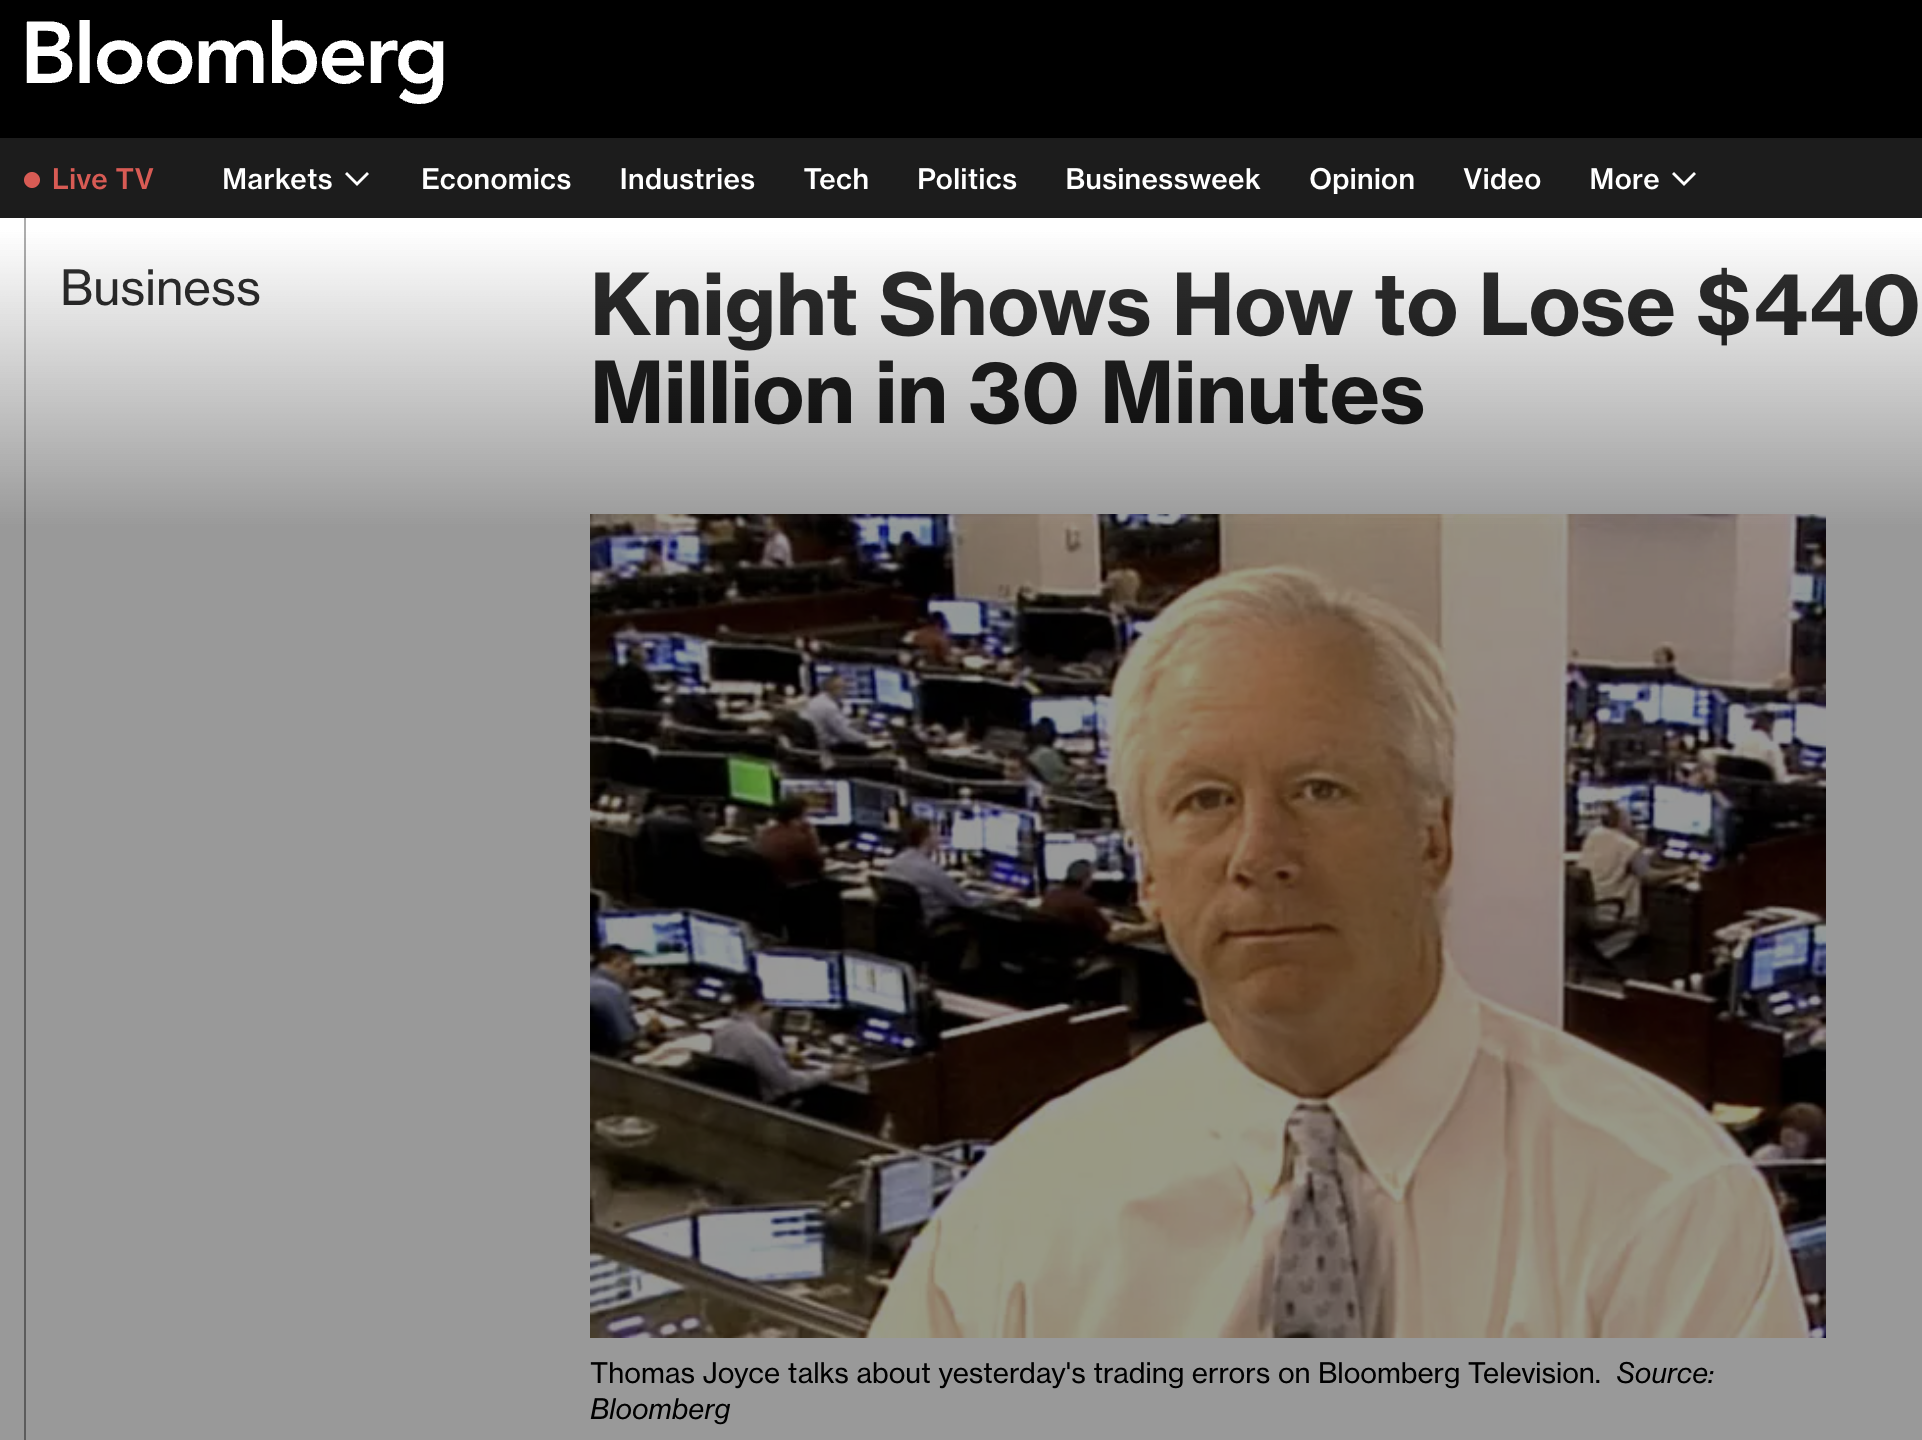
\includegraphics[width=0.6\linewidth]{figs/noticioKnight.png}
        \caption{Noticia del evento de Knight Capital Group - 1 de agosto de 2012.}
        \label{fig:placeholder}
    \end{figure}
\end{frame}

\begin{frame}{Confusión}
    Como hemos visto hasta el momento los estado mutables dificultan el trabajo de \textbf{predecir el comportamiento del programa.} Considere las siguientes preguntas:

    \begin{figure}
        \centering
        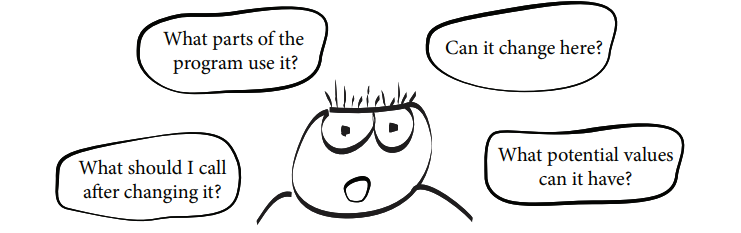
\includegraphics[width=1\linewidth]{figs/image2.png}
        \caption{La mutabilidad causa confusión.}
        \label{fig:placeholder}
    \end{figure}

    Veamos como se lidia con esto en algunos paradigmas de programación:
\end{frame}

\section{Mutabilidad en algunos paradigmas de programación}

\begin{frame}[fragile]{Nuestra solución}
    Nuestro enfoque se basó en hacer que nuestra función sea pura.
    \begin{lstlisting}[language=Java]
         static List<String> replan(List<String> plan,
                                    String newCity,
                                    String beforeCity) {
             int newCityIndex = plan.indexOf(beforeCity);
             List<String> replanned = new ArrayList<>(plan);
             replanned.add(newCityIndex, newCity);
             return replanned;
        }
    \end{lstlisting}
    Esto garantiza que no se modifique ningún valor \textbf{externo}.
\end{frame}


\begin{frame}[fragile]{POO}
    En la programación orientada a objetos probablemente usaríamos la \textit{encapsulación} para asegurar nuestra información de ser mutada de manera indeseada.

    \begin{block}{Definición}
        \textbf{Encapsulación} es una técnica que \textbf{aísla} un estado mutable, usualmente dentro de un objeto. Este objeto resguarda el estado haciendolo \textit{privado} y asegurandose que solo se interactúe con el usando la interfaz provista por la clase.
    \end{block}

     Así, la responsabilidad de manipular el estado es restringida a un solo lugar.
\end{frame}


\begin{frame}[fragile]{POO}
    En la programación orientada a objetos probablemente usaríamos la \textit{encapsulación} para asegurar nuestra información de ser mutada de manera indeseada.

     \begin{lstlisting}[language=Java]
        private List<String> plan = new ArrayList<>();
        public void replan(String newCity, String beforeCity) {
         int newCityIndex = plan.indexOf(beforeCity);
         plan.add(newCityIndex, newCity);
        }
        public void add(String city) {
         plan.add(city);
        }
        public List<String> getPlan() {
        
    \end{lstlisting}
\end{frame}

\begin{frame}{Programación Funcional}
    Simplemente no hay valores mutables.
    \begin{block}{Definición}
        \textbf{Programación funcional} es programar usando \textit{funciones puras} que manipulan valores \textit{inmutables}.
    \end{block}

    Esto garantiza que una vez un valor es creado, nunca será modificado. Si el programador necesita realizar un cambio, por más mínimo que sea, un nuevo valor necesita ser creado y el antiguo queda intacto.
\end{frame}



\begin{frame}[fragile]{Clojure}
    Veamos como se implementaría \textit{replan} usando \textbf{Clojure}:
    
\begin{lstlisting}[language=Clojure]
(defn replan [plan new-city before-city]
  (let [[cities-before cities-after] 
  (split-with #(not= % before-city) plan)]
    (concat cities-before [new-city] cities-after)))
        \end{lstlisting}

        \begin{block}{La magia de \texttt{split-with}}
        Divide la colección en dos partes usando una condición. En este caso, iteramos \textit{mientras la ciudad no sea igual a la ciudad objetivo}. Devuelve:
        \begin{enumerate}
            \item \texttt{cities-before}: Los elementos antes del corte.
            \item \texttt{cities-after}: El resto de la lista original.
        \end{enumerate}
    \end{block}

\end{frame}



\section{Aplicación en Clojure}

\begin{emptyframe}
    Aplicación en Clojure
\end{emptyframe}

\subsection{Colecciones Inmutables por Defecto}
\begin{frame}[fragile]{Colecciones Inmutables por Defecto}
    A diferencia de Java, en Clojure \textbf{todas las colecciones base son inmutables por defecto.} No tenemos que preocuparnos por hacer copias manualmente.

    \begin{itemize}
        \item \textbf{Vectores} \texttt{[]} : Colecciones indexadas.
        \item \textbf{Listas} \texttt{()} : Colecciones secuenciales.
        \item \textbf{Mapas} \texttt{\{\}} : Colecciones clave-valor (Diccionarios).
    \end{itemize}

    \vspace{0.3cm}
    \begin{center}
    
    \end{center}
\end{frame}

\subsection{Modificando Datos}
\begin{frame}[fragile]{"Modificando" Datos: Creando Copias Eficientes}
    Clojure utiliza \textit{Structural Sharing} bajo el capó para que ``modificar'' y crear copias no sea costoso en memoria.

    \begin{exampleblock}{Agregando elementos a un vector con \texttt{conj}}
        \begin{lstlisting}[language=Clojure]
user=> (def mi-vector [1 2 3])
#'user/mi-vector

user=> (conj mi-vector 4)
[1 2 3 4] ; Retorna un NUEVO vector

user=> mi-vector
[1 2 3]   ; El original permanece intacto
        \end{lstlisting}
    \end{exampleblock}
\end{frame}

\begin{frame}[fragile]{Actualizando Mapas con \texttt{assoc}}
    \begin{exampleblock}{Modificando un mapa con \texttt{assoc}}
        \begin{lstlisting}[language=Clojure]
user=> (def persona {:nombre "Ana" :edad 25})
#'user/persona

user=> (assoc persona :edad 26)
{:nombre "Ana", :edad 26} ; Retorna un NUEVO mapa

user=> persona
{:nombre "Ana", :edad 25} ; El original es inmutable
        \end{lstlisting}
    \end{exampleblock}
    
    \vspace{0.3cm}
    \begin{center}
        \textit{En Clojure, las funciones de actualización siempre retornan un nuevo valor, respetando la pureza estructural.}
    \end{center}
\end{frame}

\section{Ejercicios Prácticos}

\begin{emptyframe}
    Ejercicios Prácticos
\end{emptyframe}

\subsection{Función Pura: IVA}

\begin{frame}[fragile]{Ejercicio 1: Función Pura para calcular IVA}
    
    Sintáxis de \textit{defn}:
    
    \textbf{Objetivo:} Crear una función pura que reciba un precio y devuelva el total con el IVA (19\%) incluido.

            \begin{lstlisting}[language=Clojure]
(defn saludar []
  (println "¡Hola al semillero!"))
    \end{lstlisting}    
    
\end{frame}

\begin{frame}[fragile]{Ejercicio 1: Función Pura}
    \textbf{Objetivo:} Crear una función pura que reciba un precio y devuelva el total con el IVA (19\%) incluido.

    \begin{lstlisting}[language=Clojure]
;; Nuestra funcion pura
(defn calcular-iva [precio]
  (* precio 1.19))
;; Prueba en el REPL
user=> (calcular-iva 1000)
1190.0
user=> (calcular-iva 500)
595.0
    \end{lstlisting}
    
    \begin{block}{Definición:}
        Una función se dice \textit{pura} si cumple con:
    \begin{enumerate}
        \item \textbf{Retorna un solo valor}.
        \item \textbf{El resultado depende únicamente de sus argumentos}.
        \item \textbf{No muta ningún valor existente} (cero efectos secundarios).
    \end{enumerate}
    
    \end{block}
\end{frame}

\subsection{Estado inmutable: Usuario}

\begin{frame}[fragile]{Ejercicio 2: Sistema de Puntos}
    \textbf{Objetivo:} Definir un mapa de usuario y una función para agregarle puntos \textbf{sin mutar} el original.

            \begin{lstlisting}[language=Clojure]
(defn saludar []
  (println "¡Hola al semillero!"))
    \end{lstlisting}    
    
\end{frame}

\begin{frame}[fragile]{Ejercicio 2: Sistema de Puntos}
    \textbf{Objetivo:} Definir un mapa de usuario y una función para agregarle puntos \textbf{sin mutar} el original.

    \begin{lstlisting}[language=Clojure]
;; 1. Definimos nuestro estado inicial (inmutable)
(def usuario {:nombre "Juan" :puntos 0})

;; 2. Creamos la funcion que "actualiza"
(defn agregar-puntos [user cantidad]
  (let [puntos-actuales (:puntos user)
        nuevos-puntos (+ puntos-actuales cantidad)]
    (assoc user :puntos nuevos-puntos)))

;; 3. Comprobamos la inmutabilidad en el REPL
user=> (agregar-puntos usuario 50)
{:nombre "Juan", :puntos 50}

user=> usuario
{:nombre "Juan", :puntos 0} ; ¡El original sigue intacto!
    \end{lstlisting}
\end{frame}

\begin{frame}{Recursos y Siguiente Paso}
    \begin{block}{Para la próxima sesión...}
        Exploraremos las \textbf{Funciones como Ciudadanos de Primera Clase}. 
        Aprenderemos a tratar a las funciones como si fueran un dato más y dominaremos la trinidad de la programación funcional: \textbf{\texttt{map}, \texttt{filter} y \texttt{reduce}}.
    \end{block}

    \vspace{0.3cm}
    \begin{itemize}
        \item Crearemos y pasaremos funciones anónimas (\texttt{fn} o \texttt{\#(…)}) como argumentos.
        \item Reemplazaremos por completo la necesidad de usar bucles tradicionales.
    \end{itemize}

    \vspace{0.4cm}
    \begin{center}
        ¡Sigan practicando en \href{https://4clojure.oxal.org/}{\textbf{\texttt{4Clojure}}}!
    \end{center}
\end{frame}

\begin{emptyframe}
    ¡Gracias!
    \figure
\end{emptyframe}
\end{document}